\documentclass{article}
\usepackage{graphicx} % Required for inserting images
\usepackage[margin=0.7in]{geometry}
\usepackage{amsmath}


\title{Projekt C}
\author{Carl-Emil Rohde \\ kvb125@alumni.ku.dk}
\date{June 2023}

\begin{document}

\maketitle

\section*{Opgave 1}

\subsection*{1a}
Jeg kan starte med at splitte A op i de forskellige søjler:
$$
QR=\left(u_1\left|u_2\right| u_3\right)=\left[\begin{array}{ccc}
-5 & 1 & 1 \\
2 & 8 & 8 \\
2 & -6 & -13 \\
-4 & 12 & -16
\end{array}\right]
$$
$$
u_1=\left[\begin{array}{c}
-5 \\
2 \\
2 \\
-4
\end{array}\right] \quad u_2=\left[\begin{array}{c}
1 \\
8 \\
-6 \\
12
\end{array}\right] \quad u_3=\left[\begin{array}{c}
1 \\
8 \\
-13 \\
-16
\end{array}\right]
$$
jeg skal nu udregne værdierne i denne matrice:
$$
\left(q_1\left|q_2\right| q_3\right)=\left[\begin{array}{ccc}
r_{11} & r_{12} & r_{13} \\
0 & r_{22} & r_{23} \\
0 & 0 & r_{33} \\
0 & 0 & 0
\end{array}\right]
$$
først $r_11$ og $q_1$:
$$
\left\|u_1\right\|=\sqrt{-5^2+2^2+2^2+(-4)^2}=7
$$
$$
q_1=\frac{u_1}{r_{11}}=\frac{1}{7}\left[\begin{array}{c}
-5 \\
2 \\
2 \\
-4
\end{array}\right]
$$
Nu kan jeg beregne $r_{12}$ og $q_2$:
$$
r_{12}=q_1 \cdot u_2=\frac{1}{7} \cdot\left[\begin{array}{c}
-5 \\
2 \\
2 \\
-4
\end{array}\right] \cdot\left[\begin{array}{c}
1 \\
8 \\
-6 \\
12
\end{array}\right]=\frac{1}{7}\left[\begin{array}{c}
-5 \\
16 \\
-12 \\
-48
\end{array}\right]=-7
$$
$$
q_2^{\prime}=u_2-r_{12} \cdot q_1=\left[\begin{array}{c}
1 \\
8 \\
-6 \\
12
\end{array}\right]-(-7) \cdot \frac{1}{7}\left[\begin{array}{c}
-5 \\
2 \\
2 \\
-4
\end{array}\right]=\left[\begin{array}{c}
1 \\
8 \\
-6 \\
12
\end{array}\right]+\left[\begin{array}{c}
-5 \\
2 \\
2 \\
-4
\end{array}\right]=\left[\begin{array}{c}
-4 \\
10 \\
-2 \\
8
\end{array}\right]
$$
Jeg gik i stå med denne opgave.

\subsection*{1b}
Jeg benytter denne formel til at udregne projektionsmatricen:
$$
P=Q Q^T
$$
Jeg finder først $Q^{T}$:
$$
Q^T=\frac{1}{7}\left(\begin{array}{cccc}
-5 & 2 & 2 & -4 \\
-2 & 5 & -2 & 4 \\
2 & 2 & -5 & -4
\end{array}\right)
$$
for at finde P, tager jeg matrixproduktet:
$$
P=Q \cdot Q^T=\frac{1}{7} \cdot\left(\begin{array}{ccc}
-5 & -2 & 2 \\
2 & 5 & 2 \\
2 & -4 & -5 \\
-4 & 4 & -4
\end{array}\right) \cdot \frac{1}{7}\left(\begin{array}{cccc}
-5 & 2 & 2 & -4 \\
-2 & 5 & -4 & 4 \\
2 & 2 & -5 & -4
\end{array}\right)
$$
$$
P=\frac{1}{49} \cdot\left(\begin{array}{cccc}
33 & -16 & -12 & 4 \\
-16 & 33 & -26 & 4 \\
-12 & -26 & 45 & -4 \\
4 & 4 & -4 & 48
\end{array}\right)
$$
\subsection*{1c}
Først transponerer jeg x:
$$
x^T=\left(\begin{array}{l}
1 \\
1 \\
1 \\
0
\end{array}\right)
$$
Nu kan jeg bruge den matrice jeg fandt i delopgave b, til at opsætte følgende ligningen$P x=\operatorname{proj}_{\mathcal{U}}(x)$.
Som det næste finder jeg venstre side i denne ligning, ved at finde matrixproduktet $Px$:
$$
P x=\frac{1}{49}\left(\begin{array}{cccc}
33 & -16 & -16 & 4 \\
-16 & 33 & -16 & 4 \\
-16 & -16 & 33 & 4 \\
4 & 4 & 4 & 48
\end{array}\right)\left(\begin{array}{l}
1 \\
1 \\
1 \\
0
\end{array}\right)=\frac{1}{49}\left(\begin{array}{c}
1 \\
1 \\
1 \\
12
\end{array}\right)=\operatorname{proj}_{\mathcal{U}}(x)
$$
Nu finder jeg spejlingsmatricen $R=2 P-I$, hvilket giver mig:
$$
R=\frac{2}{49}\left(\begin{array}{cccc}
17 & -16 & -16 & 4 \\
-16 & 17 & -16 & 4 \\
-16 & -16 & 17 & 4 \\
4 & 4 & 4 & 47
\end{array}\right)
$$
Til sidste finder jeg matrix produktet:
$$
R x=\frac{2}{49}\left(\begin{array}{cccc}
17 & -16 & -16 & 4 \\
-16 & 17 & -16 & 4 \\
-16 & -16 & 17 & 4 \\
4 & 4 & 4 & 47
\end{array}\right)\left(\begin{array}{l}
1 \\
1 \\
1 \\
0
\end{array}\right)=\frac{1}{49}\left(\begin{array}{c}
-47 \\
-47 \\
-47 \\
24
\end{array}\right)=r e f l_{\mathcal{U}}(x)
$$

\subsection*{1d}
$$
\operatorname{col}(A)^{\perp}=\operatorname{null}\left(A^T\right)
$$

$$
A^T=\left(\begin{array}{cccc}
-5 & 2 & 2 & -4 \\
1 & 8 & -6 & 12 \\
1 & 8 & -13 & -16
\end{array}\right)
$$
Jeg sætter nu $A^T$ på reduceret række echelon formel. 
\\
\\
Jeg foretager rækkeoperationerne: $-\frac{1}{5} \cdot r_1 \rightarrow r_1$, $-r_1+r_2 \rightarrow r_2$, $\frac{5}{42} \cdot r_2 \rightarrow r_2$, $-r_2+r_3 \rightarrow r_3$ og får:
$$
\left[\begin{array}{cccc}
1 & -\frac{2}{5} & -\frac{2}{5} & \frac{4}{5} \\
0 & \frac{42}{5} & -\frac{28}{5} & \frac{56}{5} \\
0 & \frac{42}{5} & -\frac{63}{5} & -\frac{84}{5}
\end{array}\right]
$$
Jeg foretager rækkeoperationerne: $-\frac{1}{7} \cdot r_3 \rightarrow r_3$, $\frac{2}{5} r_3+r_1 \rightarrow r_1$, $\frac{2}{3} r_3+r_2 \rightarrow r_2$, $\frac{2}{5} r_2+r_1 \rightarrow r_1$ og får:
$$
\left[\begin{array}{llll}
1 & 0 & 0 & 4 \\
0 & 1 & 0 & 4 \\
0 & 0 & 1 & 4
\end{array}\right]
$$
Således kan må det ortogonale komplement være givet ved:
$$
\mathcal{U}^{\perp}=\left(\begin{array}{c}
-4 \\
-4 \\
-4 \\
1
\end{array}\right)
$$
da nulrummet må være den frie variabel. Som det sidste normere jeg $\mathcal{U}^{\perp}$. $\sqrt{16+16+16+1}=\sqrt{49}=7$. Den ortonormale base kan endeligt opskrives:
$$
\frac{1}{7}\left(\begin{array}{c}
-4 \\
-4 \\
-4 \\
1
\end{array}\right)
$$
\subsection*{1e}
$$
Q=\left(\begin{array}{cccc}
-5 & -2 & 2 & -4 \\
2 & 5 & 2 & -4 \\
2 & -2 & -5 & -4 \\
-4 & 4 & -4 & 1
\end{array}\right)
$$
Nu finder jeg $Q^T$ ved at transponere $Q$:
$$
Q^T=\left(\begin{array}{cccc}
-5 & 2 & 2 & -4 \\
-2 & 5 & -2 & 4 \\
2 & 2 & -5 & -4 \\
-4 & -4 & -4 & 1
\end{array}\right)
$$
Dette kan jeg gøre, fordi jeg ved at matricen er symmetrisk. Dette må nemlig betyde, at den inverse matrice må svare til $Q^T$. Nu mangler jeg bare at udregne normen af vektoren $Bv$:
$$
\|v\|=\sqrt{\sqrt{2}^2+\sqrt{5}^2+\sqrt{7}^2+\sqrt{11}^2}=\sqrt{2+5+7+11}=\sqrt{25}=5
$$
$\|B v\|$ er altså:
$$
\frac{1}{5}\left(\begin{array}{c}
\sqrt{2} \\
\sqrt{5} \\
\sqrt{7} \\
\sqrt{11}
\end{array}\right)
$$

\section*{Opgave 2}
\subsection*{2a}
For at finde en matrices egenværdier, skal vi løse det karakteristiske ligningssystem, som er givet ved determinanten af $(\mathbf{A} - \lambda\mathbf{I})$, hvor $\mathbf{I}$ er identitetsmatricen og $\lambda$ er egenværdien. Dette giver os følgende:

\begin{equation}
\begin{vmatrix}
1/2 - \lambda & 1/2 \\
-1/2 & 1/2 - \lambda
\end{vmatrix} = 0.
\end{equation}

Dette kan omskrives til:

\begin{equation}
(1/2 - \lambda)^2 - (1/2)(-1/2) = 0.
\end{equation}

Dette forenkles til:

\begin{equation}
\lambda^2 - \lambda + 1/4 + 1/4 = 0.
\end{equation}

Eller:

\begin{equation}
\lambda^2 - \lambda + 1/2 = 0.
\end{equation}

Dette er en kvadratisk ligning, som vi kan løse ved at anvende den kvadratiske formel:

\begin{equation}
\lambda = \frac{-b \pm \sqrt{b^2 - 4ac}}{2a},
\end{equation}

hvor $a = 1$, $b = -1$, og $c = 1/2$. Dette giver os:

\begin{equation}
\lambda = \frac{1 \pm \sqrt{1 - 2}}{2},
\end{equation}

Da radikanden (udtrykket under kvadratroden) er negativ, får vi komplekse løsninger. Disse er givet ved:

\begin{equation}
\lambda = \frac{1 \pm \sqrt{-1}}{2},
\end{equation}

Hvilket forenkler til:

\begin{equation}
\lambda = \frac{1 \pm i}{2},
\end{equation}
\\
\\
Så de to egenværdier for $\mathbf{A}$ er $\frac{1}{2} + \frac{i}{2}$ og $\frac{1}{2} - \frac{i}{2}$.
I den komplekse plan kan disse indtegnes som punkterne $(1/2, 1/2)$ og $(1/2, -1/2)$, hvilket repræsenterer de reelle og imaginære komponenter af egenværdierne, respektivt:
\begin{center}
    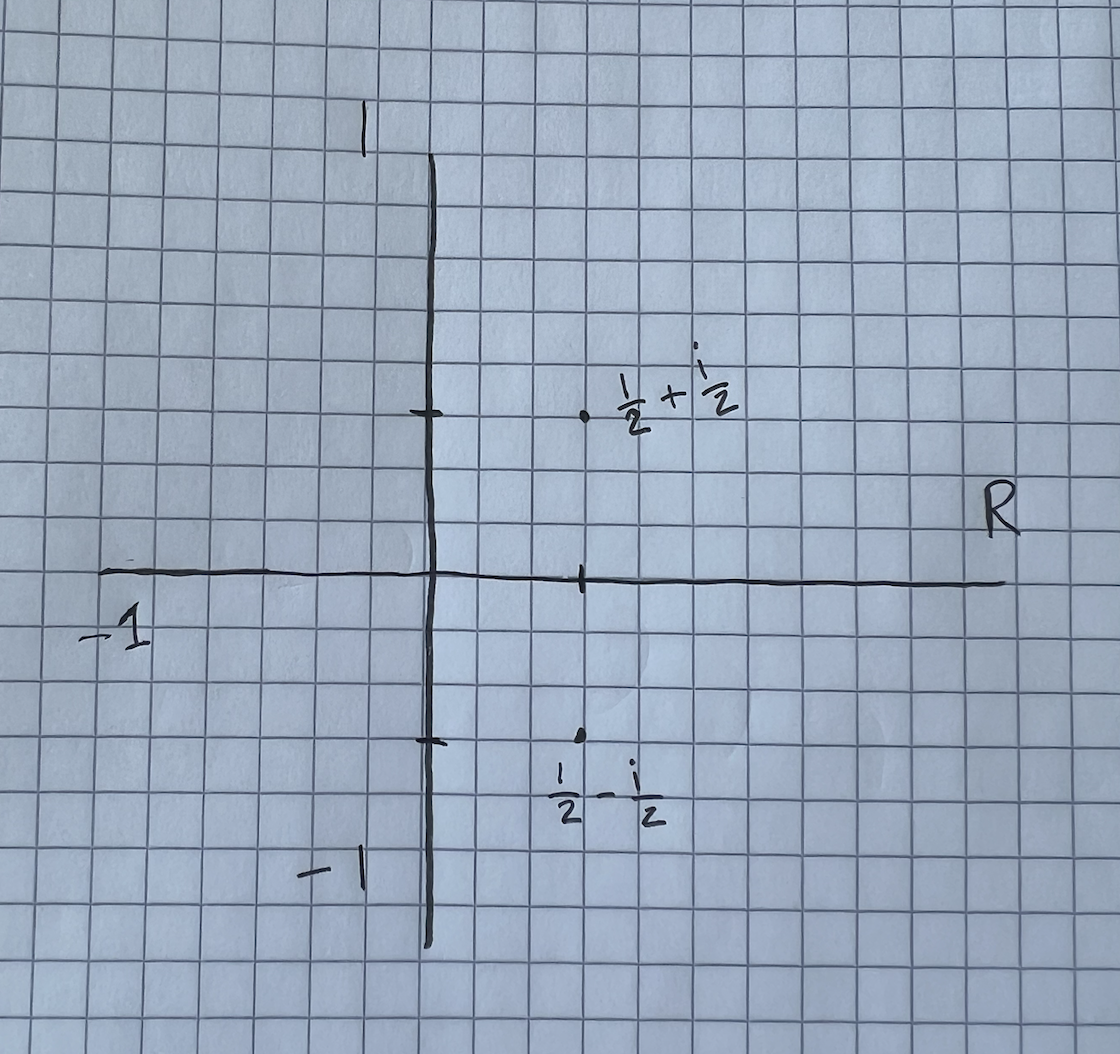
\includegraphics[scale=0.50]{po.png}
\end{center}
\subsection*{2b}
Når vi subtraherer $\lambda=\frac{1}{2}+\frac{i}{2}$ fra diagonalen af $\mathrm{A}$, ender vi med:
$$
\left[\begin{array}{cr|r}
\frac{1}{2}-\left(\frac{1}{2}+\frac{i}{2}\right) & \frac{1}{2} & 0 \\
-\frac{1}{2} & \frac{1}{2}-\left(\frac{1}{2}+\frac{i}{2}\right) & 0
\end{array}\right]=\left[\begin{array}{rr|r}
-\frac{i}{2} & \frac{1}{2} & 0 \\
-\frac{1}{2} & \frac{-i}{2} & 0
\end{array}\right]
$$
Bytter om på $r_1$ og $r_2$:
$$
\left[\begin{array}{cc|c}
-\frac{1}{2} & -\frac{i}{2} & 0 \\
-\frac{i}{2} & \frac{1}{2} & 0
\end{array}\right]
$$
multiplicere $r_1$ med $\frac{-2}{1}$:
$$
\left[\begin{array}{cc|c}
1 & i & 0 \\
\frac{-i}{2} & \frac{1}{2} & 0
\end{array}\right]
$$
$r_2$ bliver til $r_2+\left(\frac{i}{2}\right) r_1$:
$$
\left[\begin{array}{ll|l}
1 & i & 0 \\
0 & 0 & 0
\end{array}\right]
$$
Dette fører os til løsningerne:
$$
\left(\begin{array}{l}
x_1 \\
x_2
\end{array}\right)=t\left(\begin{array}{c}
-i \\
1
\end{array}\right)
$$
Så med $\lambda=\frac{1}{2}+\frac{i}{2}$ opnår vi egenrummet:
$$
E_{\frac{1}{2}+\frac{1}{2}}=\left\{\left(\begin{array}{c}
-i \\
1
\end{array}\right)\right\}
$$
Og for $\lambda=\frac{1}{2}-\frac{i}{2}$ opnår vi egenrummet:
$$
E_{\frac{1}{2}-\frac{i}{2}}=\left\{\left(\begin{array}{c}
i \\
1
\end{array}\right)\right\}
$$


\subsection*{2c}
For at finde disse værdier, løser jeg nu følgende ligningssystem:
$$
\left(\begin{array}{l}
1 \\
1
\end{array}\right)=\alpha\left(\begin{array}{l}
i \\
1
\end{array}\right)+\beta\left(\begin{array}{c}
-i \\
1
\end{array}\right)
$$
Dette kan gøres, ved at opsætte totalmatricen, og bringe den på reduceret række echelon formel:
$$
{\left[\begin{array}{cc|c}
i & -i & 1 \\
1 & 1 & 1
\end{array}\right]} \\
r_1 \leftrightarrow r_2 \\
{\left[\begin{array}{rr|r}
1 & 1 & 1 \\
i & -i & 1
\end{array}\right]} \\
r_2-i r_1 \rightarrow r_2
$$
$$
{\left[\begin{array}{cc|c}
1 & 1 & 1 \\
0 & -2 i & 1-i
\end{array}\right]} \\
\frac{i}{2} r_2 \rightarrow r_2 \\
{\left[\begin{array}{cc|c}
1 & 1 & 1 \\
0 & 1 & \frac{i}{2}+\frac{1}{2}
\end{array}\right]} \\
r_1-r_2 \rightarrow r_1 \\
{\left[\begin{array}{ll|l}
1 & 0 & \frac{1}{2}-\frac{i}{2} \\
0 & 1 & \frac{i}{2}+\frac{1}{2}
\end{array}\right]}
$$
Værdierne for alpha og beta er dermed:
$$
\alpha=\frac{1}{2}-\frac{i}{2} // \beta=\frac{1}{2}+\frac{i}{2}
$$

\subsection*{2d}
Jeg er givet følgende:
$$
V=\left(\begin{array}{l}
1 \\
1
\end{array}\right)
$$
$$
A^2=\left(\begin{array}{cc}
0 & \frac{1}{2} \\
-\frac{1}{2} & 0
\end{array}\right)
$$
$$
A^3=\left(\begin{array}{cc}
-\frac{1}{4} & \frac{1}{4} \\
-\frac{1}{4} & -\frac{1}{4}
\end{array}\right)
$$
Først udregner jeg $AV$:
$$
A V=\left[\begin{array}{cc}
\frac{1}{2} & \frac{1}{2} \\
-\frac{1}{2} & \frac{1}{2}
\end{array}\right] \cdot\left[\begin{array}{l}
1 \\
1
\end{array}\right]=\left[\begin{array}{l}
1 \\
0
\end{array}\right]
$$
Så udregner jeg $A^2 V$:
$$A^2 V=\left[\begin{array}{cc}0 & \frac{1}{2} \\ -\frac{1}{2} & 0\end{array}\right] \cdot\left[\begin{array}{l}1 \\ 1\end{array}\right]=\left[\begin{array}{c}\frac{1}{2} \\ -\frac{1}{2}\end{array}\right]$$
til sidste $A^3 V$:
$$A^3 V=\left[\begin{array}{cc}-\frac{1}{4} & \frac{1}{4} \\ -\frac{1}{4} & -\frac{1}{4}\end{array}\right] \cdot\left[\begin{array}{l}1 \\ 1\end{array}\right]=\left[\begin{array}{c}0 \\ -\frac{1}{2}\end{array}\right]$$
Nu kan jeg skitsere vektorne i XY-planen:
\begin{center}
    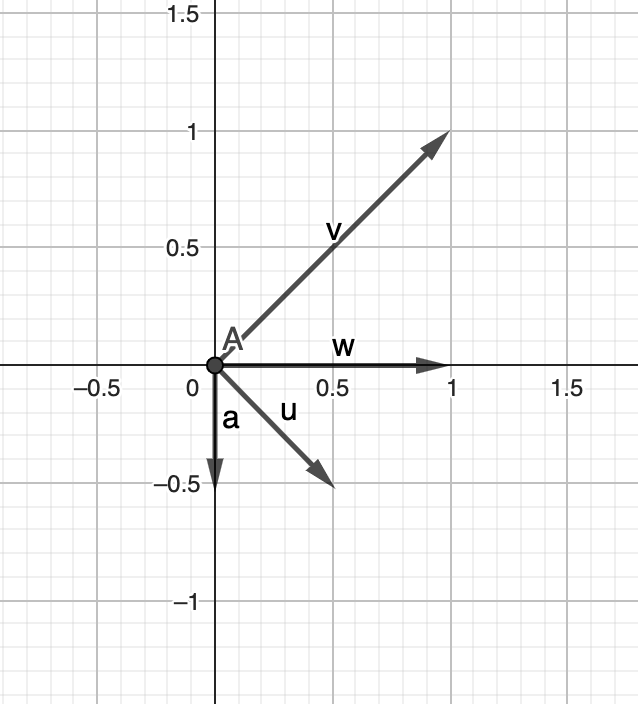
\includegraphics[scale=0.50]{vec.png}
\end{center}
Her svarer a til $A^3 V$. u til $A^2 V$. w til $AV$ og v til $V$. Alle viklerne ser ud til at være ækvivalente med 45 grader mellem dem alle.
\subsection*{2e}

\section*{Opgave 3}
\subsection*{3a}
Ud fra punkterne der er angivet i tabellen fra opgave beskrivelsen, opskriver jeg dem som forskrift for en ret linje:
$$
\begin{aligned}
& b+2010 a=35,481 \\
& b+2011 a=36,891 \\
& b+2012 a=37,331 \\
& b+2013 a=38,061 \\
& b+2016 a=39,077 \\
& b+2018 a=39,345 \\
& b+2020 a=40,568 \\
& b+2022 a=42,140 \\
& b+2023 a=43,056
\end{aligned}
$$
$$
A=\left[\begin{array}{ll}
1 & 2010 \\
1 & 2011 \\
1 & 2012 \\
1 & 2013 \\
1 & 2016 \\
1 & 2018 \\
1 & 2020 \\
1 & 2022 \\
1 & 2023
\end{array}\right]
$$
$$
x=\left[\begin{array}{l}
b \\
a
\end{array}\right]
$$
$$
b=\left[\begin{array}{l}
35,481 \\
36,891 \\
37,331 \\
38,061 \\
39,071 \\
39,345 \\
40,568 \\
42,140 \\
43,056
\end{array}\right]
$$
For at finde den bedste approksimation til konstanterne, opsætter jeg følgende:
$$
\tilde{x}=\left[\begin{array}{c}
\tilde{b} \\
\tilde{a}
\end{array}\right]=\left(A^T A\right)^{-1} A^T b=
\left[\begin{array}{c}
-966,803121 \\
0,49893480
\end{array}\right]
$$
Denne udregning er foretaget med koden fra projekt A.
\subsection*{3b}
Vi starter med vores lineære funktionsforskrift for supercomputernes FLOPS og forsøger at omformulere den til en eksponentiel form. Først isolerer vi y ved at benytte den naturlige logaritme:
$$
\ln (y)=0,499 t-966,8
$$
Herefter skriver vi y som en eksponentiel funktion ved at anvende egenskaberne for logaritmer:
$$
y=e^{\ln (y)}=e^{0,499 t+0,499(2010-2010)-966,8}
$$
Som kan simplificeres til:
$$
y=e^{-0,499(t-2010)-0,499 \cdot 2010+966,8}
$$
Til sidst beregner vi værdien af det andet eksponentielle udtryk, hvilket tillader os at skrive det endelige udtryk som:
$$
y=e^{0,499(t-2010)} \cdot 4,56 \cdot 10^{15}
$$
\subsection*{3c}
For at finde supercomputernes estimerede FLOPS i et bestemt år, indsætter jeg blot de anførte årstal i modellen fra sidste delopgave:
\\
\\
For $f(2000)$ :
$$
f(2000)=e^{0,499(2000-2010)} \cdot 4,56 \cdot 10^{15}=3,105 \cdot 10^{13}
$$
For $f(2030)$ :
$$
f(2030)=e^{0,499(2030-2010)} \cdot 4,56 \cdot 10^{15}=9,830 \cdot 10^{19}
$$

\end{document}
